\documentclass[10pt, a4paper]{article}
\usepackage{authblk} %affiliation
\usepackage{amsmath}
\usepackage{multirow} %for a multirow table
\usepackage{xcolor}
\usepackage{algpseudocode} %to write an algorithm
\delimitershortfall-1sp
\usepackage{mleftright} %for the nested brackets
\usepackage{graphicx}
\graphicspath{}
\mleftright
\renewcommand{\baselinestretch}{1.0} 
\begin{document}
	\title{Assignment}
	\author{Shashank P \\ \texttt{200010048@iitdh.ac.in}}
	\affil{Department of Computer Science, IIT Dharwad}
	\date{August 6, 2021}
	\maketitle
\newpage
\tableofcontents
\listoffigures
\listoftables
\newpage
\section{Mathematics}
In this section, various mathematical formulae and equations will be included
to include all the feature mentioned in the assignment. Very low mass particles
moving at speed less than that of light behaves like a particle and wave. De
Broglie derived an expression relating the mass of such smaller particles and its
wavelength. \par
Plank's quantum theory relates the energy of an electromagnetic wave to its
wavelength or frequency.
\begin{align} 
	E &=h\nu \notag\\ 
	&=\frac{hc}{\lambda}
\end{align}
Einstein related the energy of particle matter to its mass and velocity, as
\begin{equation} 
	E =mc^2
\end{equation}
As the smaller particle exhibits dual nature, and energy being the same, de
Broglie equated 1 \& 2 for the particle moving with velocity `v' as
\begin{equation} 
	\frac{hc}{\lambda} = mc^2 \notag
\end{equation}
Then, $\frac{h}{\lambda} = mv$ or $\lambda = \frac{h}{mv} = \frac{h}{\text{momentum}}$: `h' is the Plank's constant.We know 7 + 3 = 10.\\
We have derived this from \cite{verma2008concepts}. \\
Lets check different mathematical functions in \LaTeX			
	\subsection{Matrices}
    $\begin{bmatrix}
    	\sqrt2 & \sqrt3 & \sqrt5 \\
    	\sqrt7 & \sqrt{11} & \sqrt{13} \\
    	\sqrt{23} & \sqrt{19} & \sqrt{17}
    \end{bmatrix}$
	\subsection{Squareroot}
	Although illustrated above, we use square root again for the equation $ax^2+bx+c=0$, the roots are given by
	\begin{equation} 
		x = \frac{-b\pm\sqrt{b^2-4ac}}{2a} \notag
	\end{equation}
    This is the basic equation which study in class 10th \cite{education2016mathematics}
    \newpage
	\subsection{Integration}
	The definite integral of a continuous function $f$ over the interval $[a,b]$ denoted by $\int_a^b f(x)dx$ is the limit of a Riemann sum as the number of subdivisions
	approaches infnity. This definition is cited from \cite{ghorpade2018course}
	\subsection{Summation}
	Riemann sum can be given by:
	$$\lim_{n\to\infty} \sum_{i=0}^{n} \delta xf(x_i)$$
	\subsection{Nested brackets}
	$\left[\frac{\left(\left[\left(\left[\frac{(xy)}{z} \% w\right] +7\right) -10\right]8\right)}{\left(\left[\left(\left[\frac{(zy)}{x} \% u\right] +17\right) -1\right]5\right)}\right]$
\newpage
\begin{figure}
	\centering    
	
\includegraphics[scale=0.7]{covid}
	\caption{Graphic image}
	\label{fig:responce}
\end{figure}
\begin{table}
\begin{tabular}{|l|l|l|}
\hline
Characteristics & Chloroquine (n = 10) & P-value* \\ \hline\hline            
Age, year & 41.5 (33.8-50.0) & 0.09 \\ \hline      
Female, n (\%) & 3 (70.00) & 0.41 \\ \hline      
Days from onset to treatment & 2.50 (2.00-3.75) 6.50 & !`0.001 \\ \hline
Height, cm & 167.50 (158.00-173.00) & 0.97 \\ \hline
\end{tabular}
\caption{Treatment}
\label{tab:treat}
\end{table}
\section{Lists and figures and tables}
	\begin{itemize}
		\item A novel coronavirus disease 2019 (COVID-19) emerged around December
		2019 in Wuhan, China and has spread rapidly worldwide (Lu~et al., 2020).
		\item Until March 27, 2020, the Chinese health authorities had reported 82082
		confirmed COVID-19 cases in China with 3298 deaths and 381443 confirmed cases with 20787 deaths outside China.
	\end{itemize}
	\begin{enumerate}
		\item Coronavirus relies on cellular machinery to replicate itself, thus providing
		a rationale to search for effective therapies among agents that may impact
		pathways required for the viral life cycle.
		\item he vesicular trafficking system plays a critical role in viral entry, unpacking,
		assembly, and packaging. Among agents that can interfere with normal
		vesicular trafficking are several drugs approved for human therapies.
		\item well-known antimalaria drug, Chloroquine, stands out as one of the earliest
		reagents that can block vesicular trafficking and also interfere with the life
		cycle of parasites and viruses.
	\end{enumerate} \par
We can see from Figure \ref{fig:case} that the covid cases in India in June were already reaching high values. \\ \par 
It is evident from Figure \ref{fig:inf} that we should stay informed about covid.  \\ \par
We see table \ref{tab:treat} which shows recovery rates by chloroquinone\\
The above data is derived from research paper on covid \cite{huang2020treating}
\newpage
\begin{figure}
	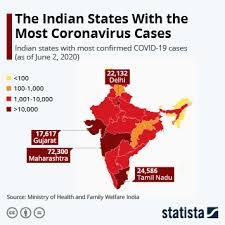
\includegraphics[width=8cm, height=8cm]{c19}
	\centering
	\caption{Cases in india}
	\label{fig:case}
\end{figure}
\begin{figure}
	
\includegraphics[scale=0.22]{cov}
	\centering
	\caption{Stay Informed}
	\label{fig:inf}
\end{figure}
\textbf{Following is description type list}
\begin{description}
	\item [CS 213] Lorem ipsum dolor sit amet,\textbf{Turned the text bold consectetur adipiscing elit, sed do eiusmod tempor incididunt} ut labore et dolore magna aliqua. \textit{Italics Ut enim ad minim veniam, quis nostrud
	exercitation ullamco laboris nisi ut aliquip ex ea commodo} . 
	\item [HS 201] Lorem ipsum dolor sit amet, consectetur adipiscing elit, sed do eius-
	mod tempor incididunt ut labore et dolore magna aliqua. Ut enim ad
	minim veniam.
\end{description}
\newpage
\pagecolor{green}
\begin{table}
	\centering
	\begin{tabular}{|c|c|c|c|c|}
		\hline
		Names & \multicolumn{2}{c|}{Maths}  & \multicolumn{2}{c|}{Science} \\
		\hline
		\multirow{2}{*}{Lorem} & X & Y & Z & W \\
				\cline{2-5}
		                       & S & R & V & U \\
		\hline
		\multirow{2}{*}{Ipsum} & 3 & 2 & 0 & 1 \\
		\cline{2-5}
		                       & T & O & P & Q \\
		\hline
		\multirow{2}{*}{Lorm}  & A & B & C & D \\
		\cline{2-5}
		                       & 2 & 3 & 1 & 0 \\
		\hline
	\end{tabular}
\caption{Scores}
\label{tab:scores}
\end{table}
\section{Fonts}
Till now we have seen \textcolor{red}{mathematical formulae} in \colorbox{blue}{section 1} and \textcolor{red}{covid data} with figures and tables in \colorbox{blue}{section 2}. In \colorbox{blue}{section 3} we will use font properties.
\begin{itemize}
	\item Bold-\textbf{This text is bold.}
	\item Italics-\textit{This text is italic.}
	\item teletype-\texttt{This text is teletype.}
	\item emphasize-\emph{This text is emphasized.}
	\item Roman-\textrm{This text is roman font family.}
	\item sans serif- \textsf{This text is sans serif font family.}
	\item slant-\textsl{This text is slant.}
	\item small capital-\textsc{This text is small capital.}
	\item uppercase-THIS TEXT IS UPPERCASE.
	\item lowercase-text is lowercase.
\end{itemize}
\par The table \ref{tab:scores} is a multi-column and multi-row table.
\newpage
\pagecolor{white}
\section{Psuedo Code}
\begin{algorithmic}
\Function{Quicksort}{$A[\,], p, r$}
	\If{$p<r$}
		\State $q \gets \textsc{Partition}(A,p,r)$
		\State \textsc{Quicksort}($A \,,p\, ,q-1$)
		\State \textsc{Quicksort}($A,\,q+1\,,r$)
	\EndIf
\EndFunction
\Function{Partion}{$A[\,], p, r$} $x \gets A[p]$ $i \gets p-1$
	\For{$j \gets p$ to $r-1$}
		\If{$A[j]<x$}
		\State $i++$
		\State swap($A[i],A[j]$)
		\EndIf
	\EndFor
	\State swap($A[i + 1],A[r]$)
	\State \Return ($i + 1$)
\EndFunction
\newline The Algorithm is derived taking hint from \cite{hoare1962quicksort}.
\end{algorithmic}
\newpage
\bibliography{test}
\bibliographystyle{ieeetr}
\end{document}